\documentclass[12pt]{article}

\title{Journal for Complex Analysis}
\author{Michael Gavina}


\usepackage{amssymb,amsfonts,amsmath,amsthm,url,graphicx}
\graphicspath{ {./images/} }


%\pagestyle{empty} % for no page numbers
\setlength{\oddsidemargin}{-.1in}      % 1in left margin
\setlength{\evensidemargin}{-.1in}     % 1in left margin (even pages)
\setlength{\topmargin}{0in}           % 1.50in top margin
\setlength{\textwidth}{6.7in}           % 6.3in text - 1.25in rt margin
\setlength{\textheight}{9in}            % Body ht for 1in margins
\addtolength{\topmargin}{-\headheight}  % No header, so compensate
\addtolength{\topmargin}{-\headsep}     % for header height and separation
%  End of margins and formatting params %
\linespread{1}
\setlength{\parindent}{0pt}


\usepackage{color}
\definecolor{cherry}{rgb}{0.9,.1,.2}
\definecolor{green}{rgb}{.2,.7,0}
\definecolor{blue}{rgb}{0,.0, .81}

\def\green#1{\textcolor{green}{#1}}
\def\cherry#1{\textcolor{cherry}{#1}}
\def\blue#1{\textcolor{blue}{#1}}

\begin{document}
\maketitle


\begin{center}
\textbf{\large Chapter 3}
\end{center}
%\noindent{\bf a} \\

\noindent{\bf Task 77} Draw a picture of $N_{1/2}(2+3i)$, the $\frac{1}{2}$-neighborhood of 2 + 3$i$. 
What can you say in general about the geometric appearance of an $\epsilon$-neighborhood?\\

\begin{center}
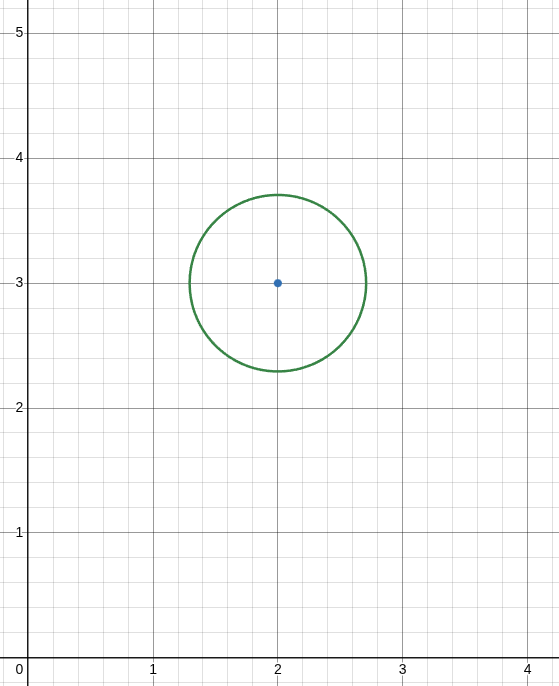
\includegraphics[scale=.5]{./images/task77.png}\\
\end{center}

Since for any given neighborhood distance, the point must be equal of N must be equal distance away the geometric shape that nieghborhoods produce is a circle.\\


\noindent{\bf Task 78} Suppose $z \in N_1(0)$, and set $\epsilon = 1 - |z|$. 
Explain why $\epsilon > 0$, and show that $N_{\epsilon}(z) \subset N_1(0)$.\\

Here $\epsilon$ is defined as $1-|z|$ and since z is in the unit circle and our given definition of neighborhoods, we know that modulus of z cannot be 1. 
This also explains that new $\epsilon$ must be greater than zero.
In addtion, the new $\epsilon$ that is created for $N_{\epsilon}(z)$ must the distance away from $N_1(0)$'s boundary.
Since this is the case, that distance must be the radius for the $N_{\epsilon}(z)$ neighborhood, which will be less than or equal to the radius of $N_1(0)$.\\


\noindent{\bf Task 79} Show that each of the following is an open subset of $\mathbb{C}$.\\


\noindent{\bf a} the upper half-plane $\mathbb{H} = \{z : $ Im$ z > 0\}$ \\

Here, if we take a point that is right above real number line, then can make an epsilon the distance from the point to the number line. 
If we then move this point closer to the number line, then we get a circle that sinks in radius. 
However, this circle will still be within $\mathbb{H}$ since we defined the epsilon as the distance from the number line below the point, then the circle will be contained within the $\mathbb{H}$ always.\\

\noindent{\bf b} the punctured plane $\mathbb{C} \ \{0\}$\\

Here, we can have the definition for epsilon be the distance from the z point to 0. 
Then any neighborhood with this epsilon can cover any point within the subset.\\

\noindent{\bf c} an annulus such as $A = \{ z : 1 < |z| < 5 \}$ \\

Since this is an annulus, this means that there is a strip in which any neighborhood could reside in.
First, we can notice that this strip has constant area and does not change across the strip. 
Then, we can find the find the point where the distance to 1 and 5 is equal. 
This point is 3, (5+1)/2 = 3.
Using this knowledge, we can make a $N_{3}(z)$ where $z \in B$, $B = {z : |z| = 3}$.\\


\noindent{\bf d} the empty set $\emptyset$ \\

For the empty set, there is nothing in the empty set so there cannot be an epsilon value.
However, since there are no values in the empty set, the condition is true automatically and thus it is an open set.\\


\noindent{\bf Task 80} Explain why each of the following subsets of $\mathbb{C}$ is \underline{not} open.\\


\noindent{\bf a} the real line $\mathbb{R} = \{ z:$ Im$ z = 0\}$ \\

Here the real number line can only contain real numbers, so when a neighborhood is described, it does not make sense.
This is because of the definition of a neighborhood, it requires the imaginary axis to capture all of the points around the points in the set.\\


\noindent{\bf b} $\{ z : -\pi < $ Im $z \leq \pi \}$ \\

This creates a strip from $-\pi$ to $\pi$, however, since the points on $\pi$ are in the set, you could have a point on that line be used as a point in a neighborhood.\\


\noindent{\bf c} ${1/n: n \in \mathbb{N}, n \neq 0}$ \\

This set has the same issue where the set is only on the real number axis, and thus cannot make a neighborhood.\\

\noindent{\bf d} $\mathbb{C} \ {1/n : n \in \mathbb{N}, n \neq 0}$ \\
This set is tricky because the set is removing the fractions where the denominator is a real numbers.
However, as the natural numbers increase in size, the distance between each fraction will be smaller and smaller.
This results in a problem where epsilon will always be greater than one, but when the limit is taken, then gap between the numbers will be zero, which epsilon cannot be.\\


\noindent{\bf Task 81} Give an example of another subset of $\mathbb{C}$ that you think is open, and show that it is.\\

Another subset that is open is the $R_+$ subset where, $R_+ = \{z :$ Re $z > 0\}$. 
This subset has to be open because if we take any point that isn't when Re z = 0, then there is a radius that can be drawn to the boundary and have that be a valid neighborhood.\\


\noindent{\bf Task 82} Determine the boundary of the open unit disk $\mathbb{D}$ and of each set in tasks 79 and 80.\\

\noindent{\bf a} $\mathbb{D}$\\

Here the boundary would be the unit circle, i.e. the points that make the circle.
Putting a neighborhood on one of these points would produce a neighborhood that contains both points in and out of the set.\\


\noindent{\bf b} The upper half-plane $\mathbb{H} = \{z:$ Im z $ > 0\}$\\

Here the boundary would be the real axis number line, any point on that line can always have points within both parts.\\


\noindent{\bf c} The punctured plane $\mathbb{C}\ {0}$ \\

Here the boundary would be zero, as it is the only point in where epsilon can be greater than it and it will still include points around it.\\

\noindent{\bf d} An annulus such as A $ = {z: 1 < |z| < 5}$\\

Here the boundary would be a circle with radius 5 centered at the origin and and the unit circle.\\

\noindent{\bf e} The empty set $\emptyset$ \\

There are no points in which the set can have a neighborhood which includes points in and outside of the set.
However, since the set contains no points, it thus contains it's boundary points and thus the boundary is its own set.\\

\noindent{\bf f} The real line $\mathbb{R} = \{z: $ Im $z = 0\}$\\

Put any neighborhood on any point in the set and it will contain both points in and out of the set, thus the boundary is its own set.\\

\noindent{\bf g} ${z: -\pi < Im z \leq \pi}$\\

Here the boundary is when Im z is equal to $-\pi$ and $\pi$.\\

\noindent{\bf h} ${1/n: n \in \mathbb{N}, n \neq 0}$\\

The boundary is the points included in the set, thus the boundary is its own set.\\

\noindent{\bf i} $C \ {1/n: n \in \mathbb{N}, n \neq 0}$\\

Here the boundary points would the points are not within the set, because placing a neighborhood on one of those points would both include points in and outside the set.\\

\noindent{\bf Task 83} Show that each of the following is a closed subset of $\mathbb{C}$.\\

\noindent{\bf a} $\mathbb{R} = {z: Im z = 0}$ \\

Here it only makes sense that this set is a closed subset because every boundary point is in the set, or better said, the points in the set are the boundary points.\\

\noindent{\bf a} $\bar{\mathbb{D}} = {z: |z| \leq 1}$\\

Since the modulus of z can be equal to 1, it is possible for points to lie on the unit circle and those points would be in the set.\\

\noindent{\bf a} $\mathbb{C}$\\

There is no boundary to the set, so it includes its set of the empty set.\\

\noindent{\bf a} $\emptyset$\\

There are no points within the empty set, and thus it includes itself.\\


\noindent{\bf Task 84} Give an example of a subset of $\mathbb{C}$ that is neither open nor closed.
Explain why neither condition holds.\\

Task 80 has a subset where the set is neither open nor closed, ${z: -\pi < Im z \leq \pi}$. 
This is the case because either side could be approached and reach a different conclusion about the set.
There are some points where points are included and when nieghborhoods are drawn, they includes points outside the set.
There are other points where points are not included and can only ever be approached.\\


\noindent{\bf Task 85} Find the closure of each of the sets in tasks 79, 80, and 84.\\

\noindent{\bf a} $\mathbb{D}$\\

Here the closure would be the set that includes its boundary points, 
this would be the unit circle.\\

\noindent{\bf b} The upper half-plane $\mathbb{H} = \{z:$ Im z $ > 0\}$\\

Since the points on the real number axis are not included, these would be the boundary points. 
Adding the real axis to the points would provide the closure set.\\

\noindent{\bf c} The punctured plane $\mathbb{C}\ {0}$ \\

Here since zero is the boundary of the open set, simply including it would provide the closure.\\

\noindent{\bf d} An annulus such as A $ = {z: 1 < |z| < 5}$\\

Here the annulus would have two different sets of boundary points, one on the circle of radius 1 and another on the circle of radius 5.
Unioning both circles would provide the closure of the set.\\

\noindent{\bf e} The empty set $\emptyset$ \\

Here the empty set closure would be the empty set because the set includes its own boundary points.\\

\noindent{\bf f} The real line $\mathbb{R} = \{z: $ Im $z = 0\}$\\

Here the closure would be the set.
This would have to be the case because the set already contains points in which the neighborhood would have points inside and outside of the set.\\

\noindent{\bf g} ${z: -\pi < Im z \leq \pi}$\\

Here half of the set already has a closure property, since when Im z $ \leq \pi$ it also includes $\pi$. 
However, $-\pi$ is not included, and thus are boundary points that do not have a closure property. 
Thus, the closure would simply add Im z $> -\pi$ to the set to have its closure.\\

\noindent{\bf h} ${1/n: n \in \mathbb{N}, n \neq 0}$\\

Here the set already has its own boundary points included in the set.
This is because when a neighborhood is applied to any point on the set, then it will include points inside and outside of the set.\\

\noindent{\bf i} $C \ {1/n: n \in \mathbb{N}, n \neq 0}$\\

Here the boundary points are the points of the set ${1/n: n \in \mathbb{N}, n \neq 0}$, however, adding these points to the set would result in a $\mathbb{C}$ set.
Thus the closure for this set is $\mathbb{C}$.\\


\noindent{\bf Task 86} Determine whether each of the following sequences converges, and if so, to what limit.\\

\noindent{\bf a} $z_n = i^n$ \\

This limit does not converge.
This will spin around the unit circle, from 1 to i to -1 to -i back to 1 which means that any one on these points could the L, which does not make sense.\\

\noindent{\bf b} $z_n = i^n/n$ \\

Here the limit does converge to 0.
The best way to look at this is with the polar form representation, $ \frac{1^n(\cos(n\theta) + i\sin(n\theta)}{2^n}$.
Here since the magintude of i is always 1, then the denominator will grow infinately large and approach 0.
Thus the limit for this expression is 0.\\

\noindent{\bf c} $z_n = (\frac{1+i}{2})^n$ \\

Here the denominator will grow faster than the numerator and thus the limit will be 0.\\

\noindent{\bf d} $z_n = (1 - i\sqrt{3})^n$\\

Since the limit is being taking over all of the complex number, the magintude of the number will always grow, and thus will never approach anything.\\

\noindent{\bf e} $z_n = 1 - (\frac{i}{\sqrt{2}})^n$\\

Since we can show that $\frac{1}{\sqrt{2}}^n$ approach 0, then $(\frac{i}{\sqrt{2}})^n$ would also approach 0.
Thus the term would be removed and the limit would converge to just 1.\\

\noindent{\bf f} $z_n = (\frac{3}{5} + \frac{4}{5}i)^n$\\

In polar coordinates, the $1^n(\cos(n\theta) + i\sin(n\theta)$, thus as n approaches infinity, the magnitude would never change, and the angle would only be multiples of the original angle.\\


\noindent{\bf Task 87} Suppose $ \lim_{n\to\infty} z_n = L_1$ and $\lim_{n\to\infty} w_n = L_2$.  
Use Theorem 1 and convergence properties of sequences of real numbers to explain why 
$\lim_{n\to\infty} (z_n + w_n) = L_1 + L_2$ and $\lim_{n\to\infty} z_nw_n = L_1L_2$.\\

For $\lim_{n\to\infty} (z_n + w_n) = L_1 + L_2$, 
lets have $z_n = x_n + y_ni$ and $w_n = u_n + v_ni$.
By Theorem 1, Re $L_1 = \lim{n\to\infty} x_n $, Im $L_1 = \lim_{n\to\infty} y_n$, Re $L_2 = \lim{n\to\infty} u_n$, Im $L_1 = \lim_{n\to\infty} y_n$.\\

Then, $z_n + w_n = x_n + y_ni + u_n + v_ni = (x_n+u_n) + i(y_n+v_n)$, which then means we can take the real part and the imaginary parts of both to get:
$\lim_{n\to\infty} (x_n+u_n) = $Re $ L_1 + L_2$, and $\lim_{n\to\infty} (y_n+v_n) = $Im $ L_1 + L_2$.
Due to this, with both parts, Theorem 1 makes both parts again. 
Thus $\lim_{n\to\infty} (z_n + w_n) = L_1 + L_2$. 


For $\lim_{n\to\infty} (z_nw_n) = L_1L_2$,
Similiarly we can break things up into the real and imaginary parts of both limits.
$\lim_{n\to\infty} ((x_n+y_ni)(u_n+v_ni)) = (x_nu_n - y_nv_n) + i(x_nv_n + y_nu_n)$.
Here, then the Re $L_1L_2 = x_nu_n - y_nv_n$ and the Im $L_1L_2 = x_nv_n = y_nu_n$. 
By Theorem 1, both parts make the whole so, $\lim_{n\to\infty} (z_nw_n) = L_1L_2$.\\


\noindent{\bf Task 88} \\

\noindent{\bf a} Find sequences $z_n$ and $w_n$ such that $\lim_{n\to\infty} (z_n + w_n)$ exists but $\lim_{n\to\infty} z_n$ and  $\lim_{n\to\infty} w_n$ do not.\\

If we define $\lim_{n\to\infty} z_n = (1 + \sqrt{3}i)^n$ and $\lim_{n\to\infty} w_n = -(1 + \sqrt{3}i)^n$, then they will spiral out forever.
However, when we add them, they cancel out to zero wil means that their limit would be zero.\\

\noindent{\bf b} Find sequences $z_n$ and $w_n$ such that $\lim_{n\to\infty} z_nw_n$ exists but $\lim_{n\to\infty} z_n$ and  $\lim_{n\to\infty} w_n$ do not.\\

If we define $\lim_{n\to\infty} z_n = i^n$ and $\lim_{n\to\infty} w_n = (\frac{1}{i})^n$ then neither of these limits exist because they will spin around the unit circle.
However, if we multiply them together, we get 1 as the value and when that is taken to the infinity it will just be 1.\\


\noindent{\bf Task 89} Suppose $B \subset \mathbb{C}$ is closed. Show that if $z_1,z_2,z_3,...$ is a sequence of points in B that converges to a limit L, then $L \in B$.\\

Lets assume that $B \subseteq \mathbb{C}$ and is closed.\\

Proof by contradiction.\\
Lets say that $L \not\in B$.
Then definition 3.3.1 states, a sequence in $\mathbb{C}$ is a function $N_+ \mapsto \mathbb{C}$. In other words, it is an ordered list of numbers $z_1,z_2,z_3,...,$ called \textit{terms} of the sequence. 
A sequence \textit{converges} to the \textit{limit} L if for every $\epsilon > 0$ there exist $n_0 \in \mathbb{N}$ such that $z_n \in N_{\epsilon}(L)$ for all $n > n_0$. 
If such a number L exists, we write $\lim_{n\to\infty} z_n = L$.
Given as such since, since our sequence of points do converge onto L and every $z_n$ is within B, then L must be a boundary point.
Definition 3.2.1. defines boundary points as points where $N_{\epsilon}(L)$ contains both points inside and outside the circle.
However, B is closed, so L must be contain within B.
QED.\\


\noindent{\bf Task 90} Use Definition 3.4.1. and the results of task 87 to show the following.\\

\noindent{\bf a} If $a,b \in \mathbb{C}$ are constants, then $\lim_{z \to z_0} (az+b) = az_0 + b$.\\

If we say that $f(z) = az + b$, then with Definition 3.4.1. we can say that $\lim_{z\to z_0} z_n = z_0$ is true and that $f(z_0) = w_0$ where $w_0 = az_0 + b$.\\

\noindent{\bf b} $\lim_{z \to z_0} z^n = z^{n}_{0}$ for all $n \geq 1$.\\

With the limit, we can say that $f(z) = z^n$, then we can say $\lim_{z\to z_0} z^{n-1}z = z^{n-1}z_0$.

Proof by induction.\\

Base case: $\lim_{n\to z_0} z^n = z^{n-1}z = z^{n-1}z_0$.\\
Hypothesis: $\lim_{n \to z_0} z^{n-k}z^k_0$\\
Inductive Reasoning: $\lim_{n \to z_0} z^{n-k}z^k_0 = z^{n-k-1}z^{k+1}_0$\\


\noindent{\bf Task 91} Determine whether each of the following limits exists, and if so what number it equals.\\

\noindent{\bf a} $\lim_{z \to 1+i} iz^2 - 2\bar{z} + 1$ \\
The limit can just be plugged within the equation.\\
$i(1+i)^2 - 2(1-i) + 1$\\
$i(1-1 + 2i) - 2 + 2i + 1$\\
$i(2i) - 1 + 2i$\\
$-2 - 1 + 2i$\\
$-3 + 2i$\\

\noindent{\bf b} $\lim_{z \to i} \frac{z^2 + 1}{z-i}$ \\
$\lim_{z \to i} \frac{z^2+1}{z-i}$\\
$\lim_{z \to i} \frac{(z-i)(z+i)}{z-i}$\\
$\lim_{z \to i} (z+i)$\\
$2i$\\


\noindent{\bf c} $\lim_{z \to 1+2i} |z|$ \\
This limit is simply the modulus of 1+2i.\\
$\lim_{z \to 1 + 2i} |z|$\\
$|1+2i| = \sqrt{5}$\\


\noindent{\bf d} $\lim_{z \to 0} \frac{\bar{z}}{z}$ \\
This limit does not exist, if you approach it from the imaginary axis, you get the answer to be -1. 
If you approach it from the real axis, you get 1.\\

\noindent{\bf e} $\lim_{z \to 1} \frac{|z|-1}{z-1}$ \\
This limit does not exist, if you apporach it from the real axis you get 1, from the imaginary axis you get 0.\\

\noindent{\bf f} $\lim_{z \to 0} (\frac{\bar{z}}{z})^2$ \\
This limit does not exist, I did this in polar coordinates:\\
$z = r(\cos(\theta) + i\sin(\theta))$, $\bar{z} = r(\cos(\theta) - i\sin(\theta))$\\

For $\frac{\bar{z}}{z}$ we get the cosines and sines on the top and bottom, but what is the angle of 0? 
This question does not make sense, so this limit does not exist.\\

\noindent{\bf Task 92} \\

\noindent{\bf a} Explain why $z \mapsto \bar{z}$ is continuous.\\

Here the function is continous because there are no holes, jumps, or asymptotes on the graph.
We can plug in $z = a + bi$, where $a,b \in \mathbb{Q}$, and no gaps or holes will appears.\\

\noindent{\bf b} Explain why $z \mapsto z^2$ is continuous.\\

Similiarly, we can take the same steps as in the last probelm, $z = a + bi$ where $a,b \in \mathbb{Q}$ to find no holes, jumps or asymptotes.\\

\noindent{\bf c} Explain why $z \mapsto \sqrt{z}$ is not continuous.\\

If we take a look at the square root of -1, we see that we get i. 
However, if we take points just above and below -1, we see that we get points very close to i and -i respectively. 
This means that as the limit approaches either side of -1, we will get two different values until we get onto -1 in which we will get i.
This means a jump or discountinuous point on the graph of the function appears.
Thus, the function is not continuous.\\


\noindent{\bf Task 93} Find an open subset U of $\mathbb{C}$, as large as possible, on which $z \mapsto z^2$ is one-to-one.
What is the image of U? Call this image V. 
How can you tell that $z \mapsto \sqrt{z}$ is continuous on V?\\

Lets label U as $\{z : $ Im$ z > 0, $ Re $z > 0 \}$.
This will produce an image V that will still be $\{z : $ Im$ z > 0, $ Re $z > 0 \}$.
Given this, since the function is one to one, there can only be one input and one output, so we can take the princple square root here since Re z and Im z > 0.
Thus, the $z \mapsto \sqrt{z}$ must be continuous on that subset.\\

\end{document}
